%&tex
\documentclass{beamer}

\usepackage{graphicx}

\usepackage{cleveref}
\usepackage{subcaption}
% \usepackage[dvipsnames]{xcolor}
\usepackage{xcolor}

\title{\(C_D\) estimation using SI-PINN \\ with multi-frequency sampled data \\ and \\ comparison with Least-Squares}

\begin{document}

\begin{frame}
	\maketitle
\end{frame}

%------------------------------------------------------------------------------
\begin{frame}
	\frametitle{Governing Equation}

	\begin{align*}
		\frac{dV}{dt} &= -\frac{\bar{q}S}{m}C_D + \frac{T}{m}cos(\alpha) + g sin(\alpha - \theta)
	\end{align*}

	\vspace{0.5cm}

	\begin{align*}
		\frac{dV}{dt} &= f\left(V, \alpha, \theta, C_D\right)
	\end{align*}

	\vspace{0.5cm}

	\begin{align*}
		C_D = C_{D_0} + C_{D_{\alpha}} \alpha + C_{D_{\delta_e}} \delta_e
	\end{align*}

\end{frame}

%------------------------------------------------------------------------------
\begin{frame}
	\frametitle{Model Schematic}
	\begin{figure}
		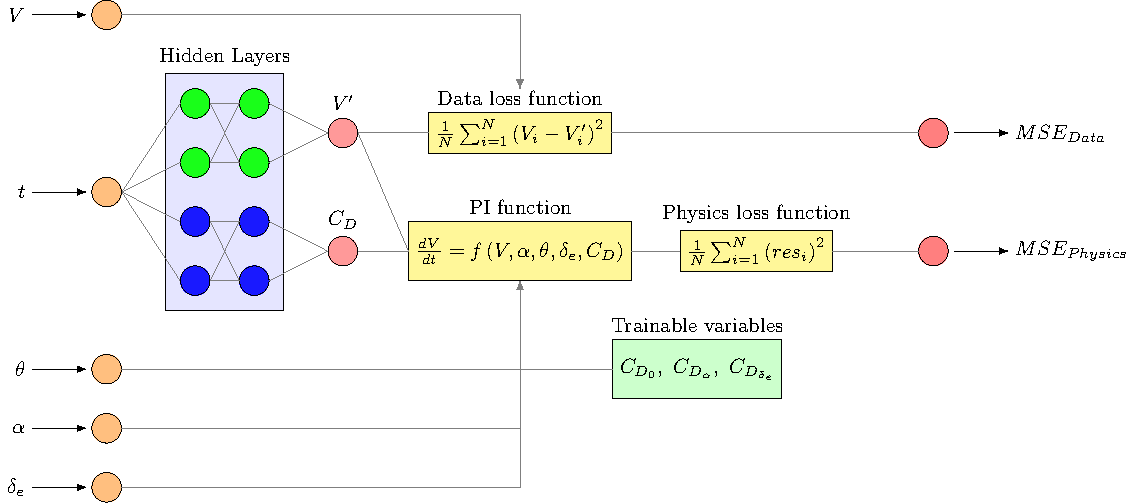
\includegraphics[scale=0.6]{01_schematic/SIPINN_schematic_V.pdf}
	\end{figure}
\end{frame}

%------------------------------------------------------------------------------

\begin{frame}
	\frametitle{Key Points}
	\begin{itemize}
		\item MSE loss function is used.
			\vspace{0.75cm}
		\item synthetic data is generated by using smoothed \(\delta_e\)
			\vspace{0.75cm}
		\item V data is sampled at 6.3 Hz (93 points/14.78s) and other state variables at 12.5 Hz (185 points/14.78s)
			\vspace{0.75cm}
		\item V-network is trained with down-sampled V data and CD network is trained with 185 points of other state variables
			\vspace{0.75cm}
		\item The results are compared with Least-Squares estimate for same 6.3 Hz data
	\end{itemize}
\end{frame}

%------------------------------------------------------------------------------
\begin{frame}
	\frametitle{Results: V prediction down-sampled data}
	\begin{figure}
		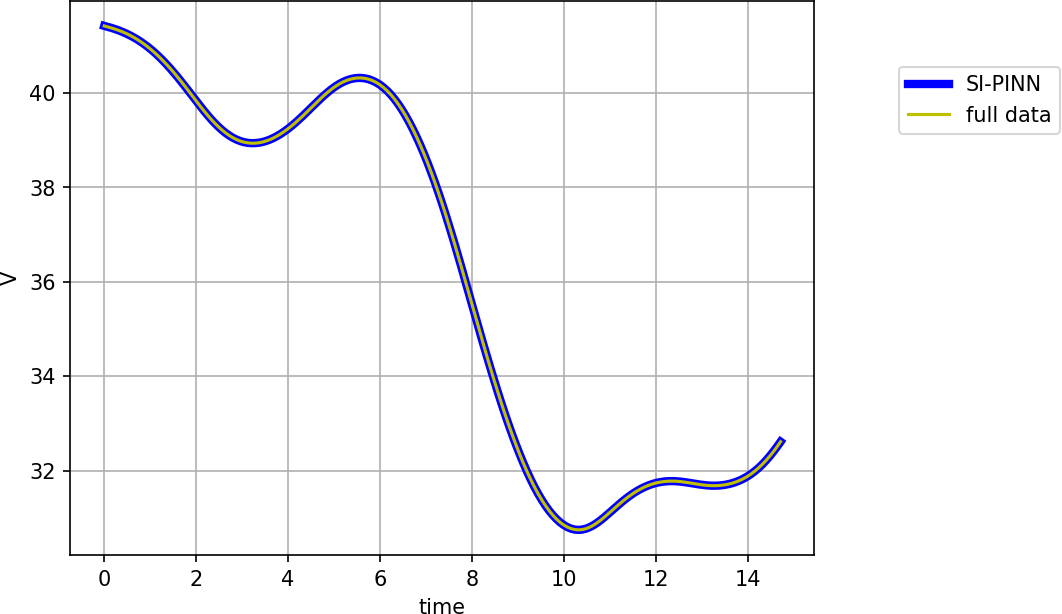
\includegraphics[scale=0.5]{supportingFiles/V_comparison.png}
	\end{figure}
	V-network is trained with 93 data points and predicted for the 185 data points
	\textcolor{blue}{blue} range. \textcolor{yellow}{Yellow} line is actual 185 data points curve.
\end{frame}


\begin{frame}
	\frametitle{Results: prediction graphs}
	\begin{columns}
		\begin{column}{0.5\linewidth}
			\begin{figure}
				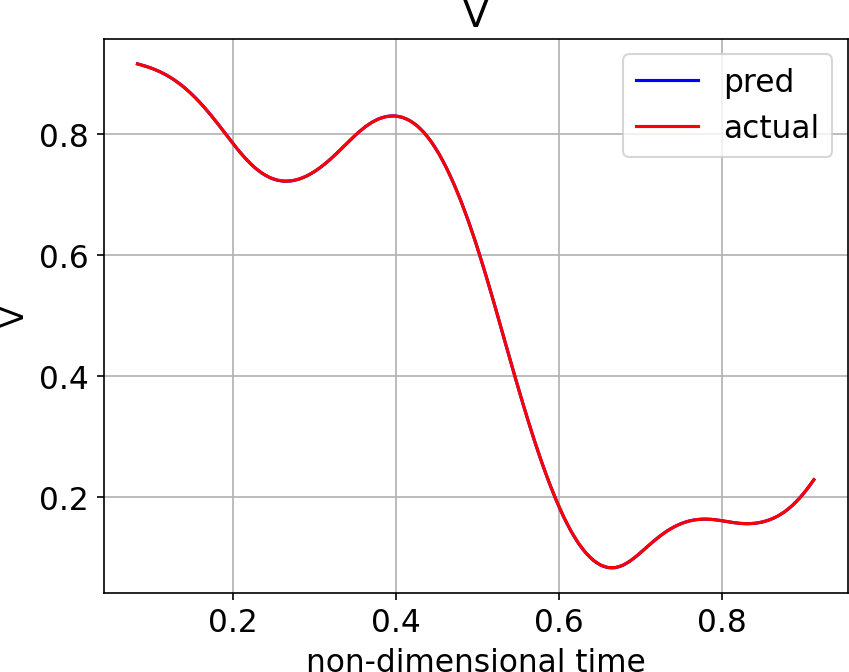
\includegraphics[scale=0.35]{supportingFiles/V.png}
			\end{figure}
		\end{column}
		\begin{column}{0.5\linewidth}
			\begin{figure}
				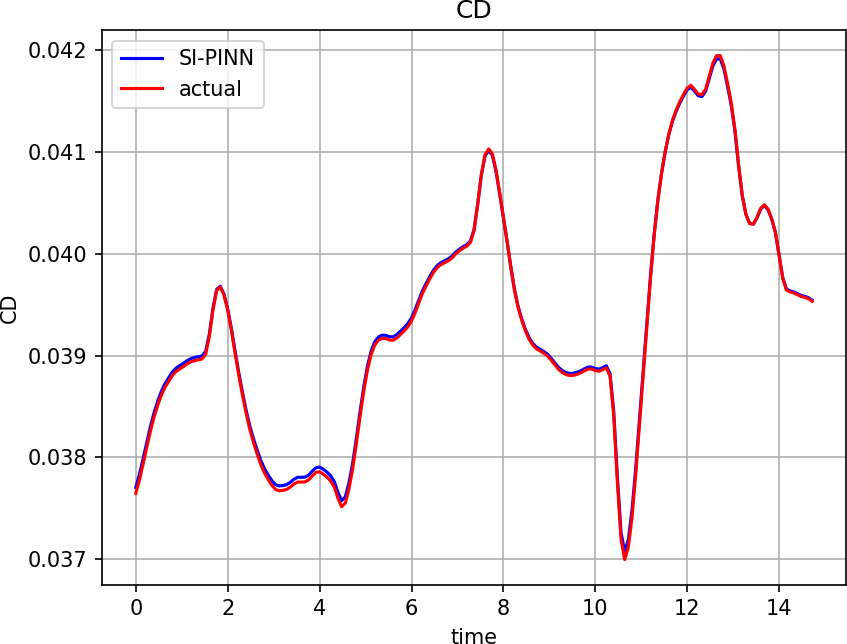
\includegraphics[scale=0.35]{supportingFiles/CD_output.png}
			\end{figure}
		\end{column}
	\end{columns}
	\begin{figure}
		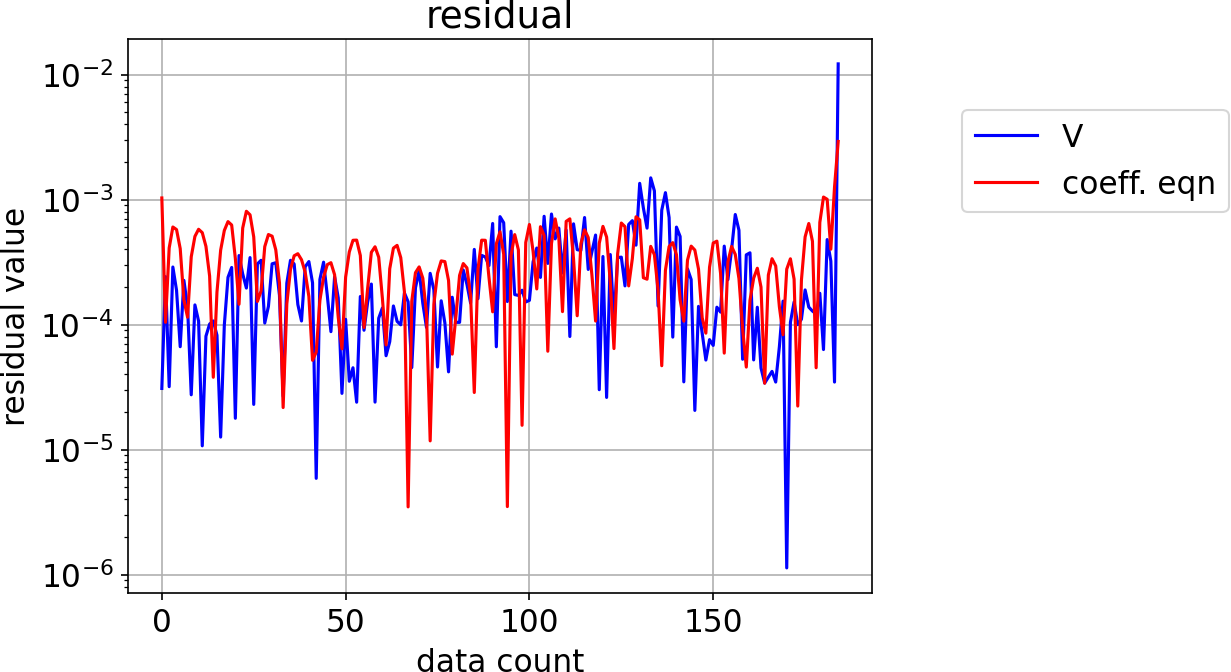
\includegraphics[scale=0.35]{supportingFiles/residual.png}
	\end{figure}
\end{frame}

\begin{frame}
	\frametitle{Results: Estimation with down-sampled data points on V}

	\begin{table}
		\caption{SI-PINN computed values}
		\begin{tabular}{|c|c|c|c|}
		\hline
			coefficient & predicted value & actual value & error percentage \\ \hline \hline
			\(CD_0\)        &  0.0360884       & 0.036         & 0.245           \\ \hline
			\(CD_\alpha\)   & 0.0401513        & 0.041         & 2.07           \\ \hline
			\(CD_{\delta_e}\)     &  0.0250605      & 0.026       & 3.61          \\ \hline
		\end{tabular}
	\end{table}

	\begin{table}
		\caption{Least-Squares computed values}
		\begin{tabular}{|c|c|c|c|}
		\hline
			coefficient & predicted value & actual value & error percentage \\ \hline \hline
			\(CD_0\)        &   0.0370633      & 0.036         & 2.95            \\ \hline
			\(CD_\alpha\)   &  0.0292532       & 0.041         & 28.65           \\ \hline
			\(CD_{\delta_e}\)     & 0.0114898       & 0.026       & 55.80          \\ \hline
		\end{tabular}
	\end{table}

\end{frame}

%------------------------------------------------------------------------------

\begin{frame}
	\frametitle{Observations}
	\begin{itemize}
		\item SI-PINNs show better estimation with multi-frequency sampled data than least squares
			\vspace{1cm}
		\item LS has to be evaluated at the least frequency of available points without
			pre-processing. But SI-PINN do not need that
	\end{itemize}
\end{frame}


\end{document}
